% !TeX spellcheck = en_US
\addscenariosection{1}{Cooperative scenario}{Emerald Island - Scavenger Hunt}{\images/logistics.png}

\begin{multicols*}{2}

\textbf{Author:} Invoceusse

\textbf{Source:} \href{https://discord.com/channels/740870068178649108/1222679455261261986}{Archon Studio Discord}

\textit{Lord Markham has decided to organise a treasure hunt and you and your friends are going to take part.
  But hurry up! Other teams are also on the trail, and one of them is almost finished!
  And above all, beware: it seems that on this island lurks a creature identified as a dragon!}
\subsection*{\MakeUppercase{Scenario Length}}

This scenario is played over 8 rounds.

\subsection*{\MakeUppercase{Player setup}}

\textbf{Player Count:} 1 - 4

\textbf{Starting Resources:}\par
\resources{5}{2}{1}

\textbf{Starting Income:}\par
\resources{10}{0}{1}

\textbf{Starting Units:}
\begin{itemize}
  \item A Pack of \svg{bronze} units of your choice.
  \item A Few \svg{bronze} units of your choice.
\end{itemize}

\textbf{Town Buildings:} \svg{bronze} Dwelling

\textbf{Map tile Pool:} If you wish, you can have the II-III tiles distributed equally to each player rather than laying them out as proposed.

\textbf{Additional Bonus:} None

\subsection*{\MakeUppercase{Map Setup}}

Take the following Map tiles and set them up as shown in the scenario map layout (P for the number of players):

\textbf{(1*P) Starting (I) Map tile}
\begin{itemize}
  \item Starting Tiles of your chosen factions.
  \item Ignore any yellow line between tiles I (but not between tiles I and tiles II-III)
\end{itemize}

\textbf{(4*P) × Far (II-III) Map tile}

\textbf{0 × Near (IV-V) Map tile}

\textbf{0 × Center (VI-VII) Map tile}

\subsection*{\MakeUppercase{Victory Conditions}}

Flag all mines and settlements. (Don't forget the mine of building materials in tile I, and each tile II-III are one mine (or settlements) with III fight)

\subsection*{\MakeUppercase{Defeat Conditions}}

There are unflagged mines or settlements left in map at the end of Round 8.

\subsection*{\MakeUppercase{Timed Events}}

\textbf{5$^{th}$ Round:}
\begin{itemize}
  \item gain again the result of one field with black cube.
\end{itemize}

\subsection*{\MakeUppercase{Additional Rules}}
\begin{itemize}
    \item cannot build gold dwelling.
    \item You can give units, even outside your turn, to another player if one of your heroes is:
    \begin{itemize}
        \item In the same tile. 
        \item In their castle.
        \item Next to it.
    \end{itemize}
    \item If you have no unit in your unit deck (after a battle or if you not keep at least one unit) return all your unit to your faction's unit (even if other player are one or more of your unit).
    \item When on another player's castle, you may recruit or reinforce their units, for them or for yourself (You may only do so if they have built the corresponding dwelling/citadel) if the other player are agreed with that.
    \item For the last mine/settlement battle add a gold neutral unit. (you have unlimited turns for this battle.) You can't use expert diplomacy to skip this battle!
    \item The first time you reach the level IV, gain your second specialty.
    \item When you reach level IV, move your token in level tracker to level III.
    \item Additionally, no player can:
    \begin{itemize}
        \item Attack other Heroes.
        \item Capture a Mine or Settlement that is already controlled.
    \end{itemize}
\end{itemize}

\vspace{3em}

\begin{center}
  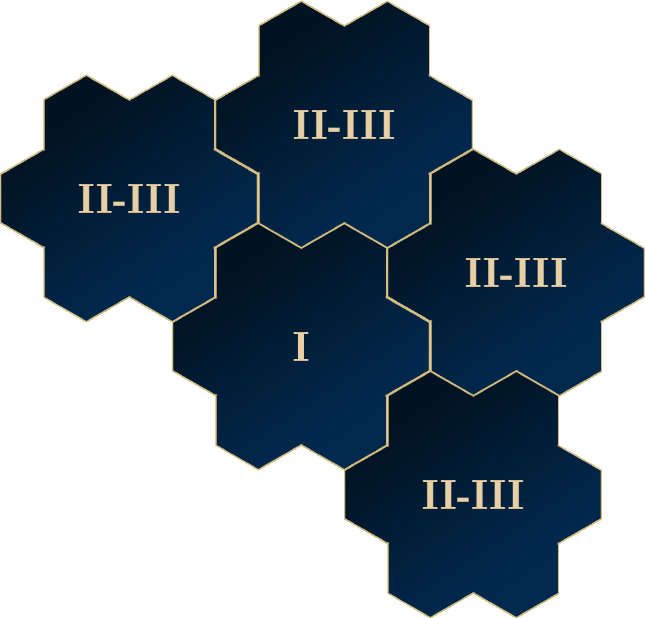
\includegraphics[width=0.2\paperwidth]{\_assets/maps/emerald-1.png}
  \captionof{figure}{1-PLAYER SCENARIO}
  \vspace{3em}
  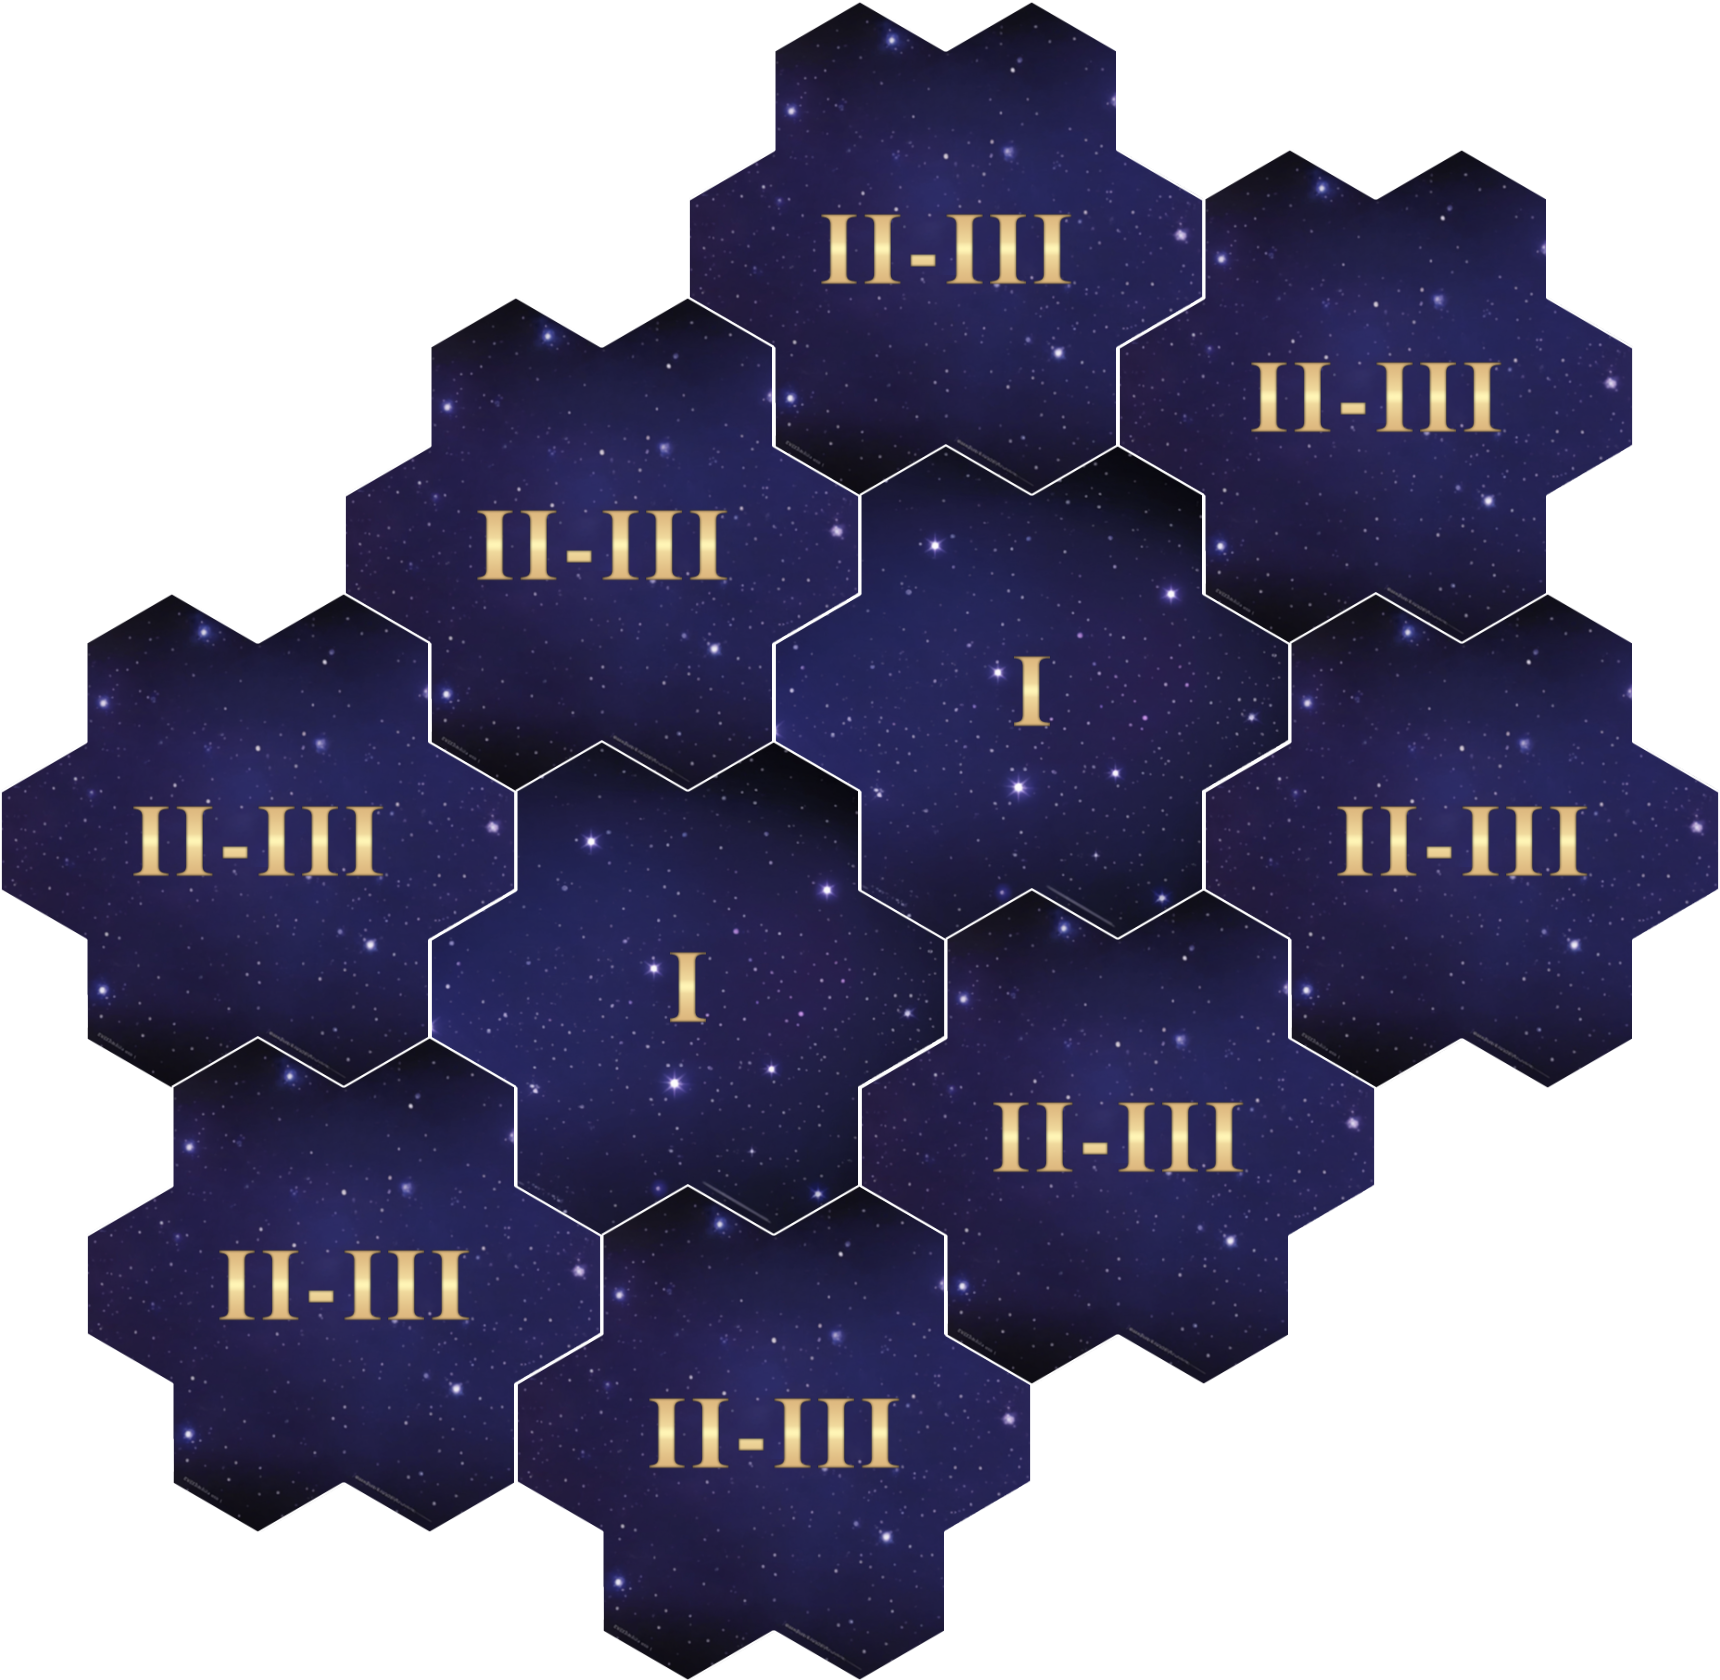
\includegraphics[width=0.3\paperwidth]{\_assets/maps/emerald-2.png}
  \captionof{figure}{2-PLAYER SCENARIO}
  \vspace{3em}
  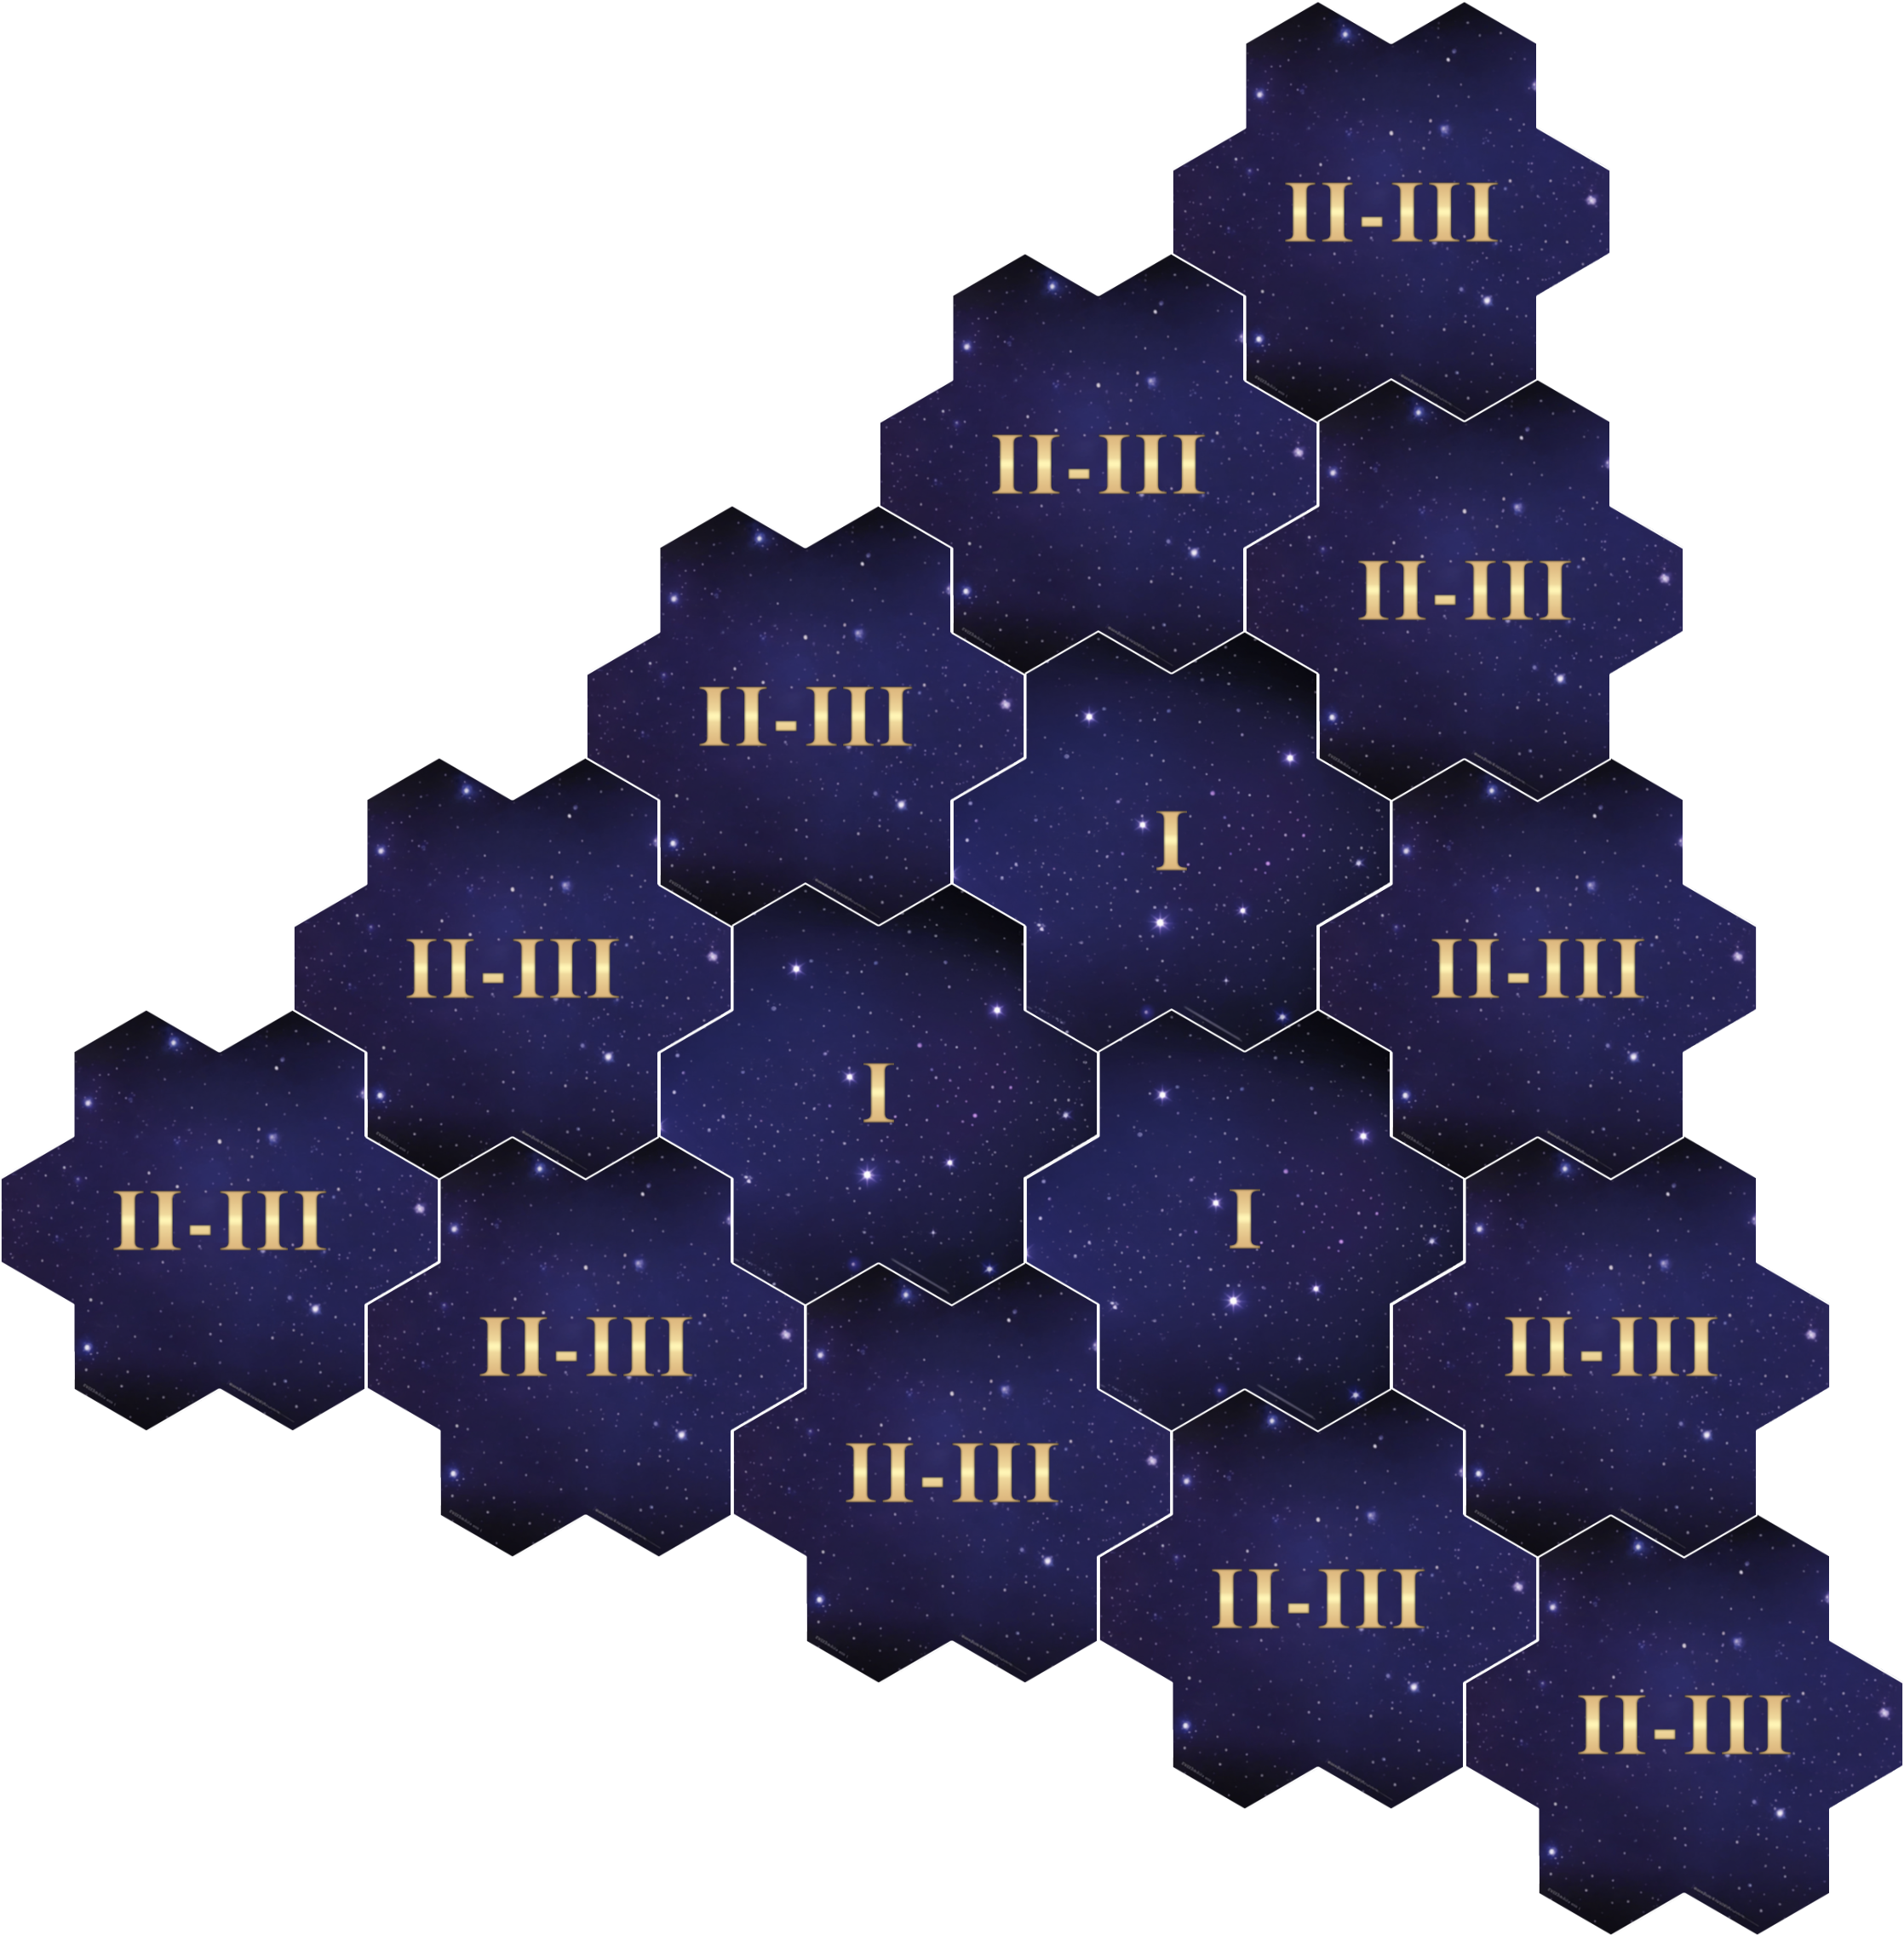
\includegraphics[width=0.3\paperwidth]{\_assets/maps/emerald-3.png}
  \captionof{figure}{3-PLAYER SCENARIO}
  \vspace{3em}
  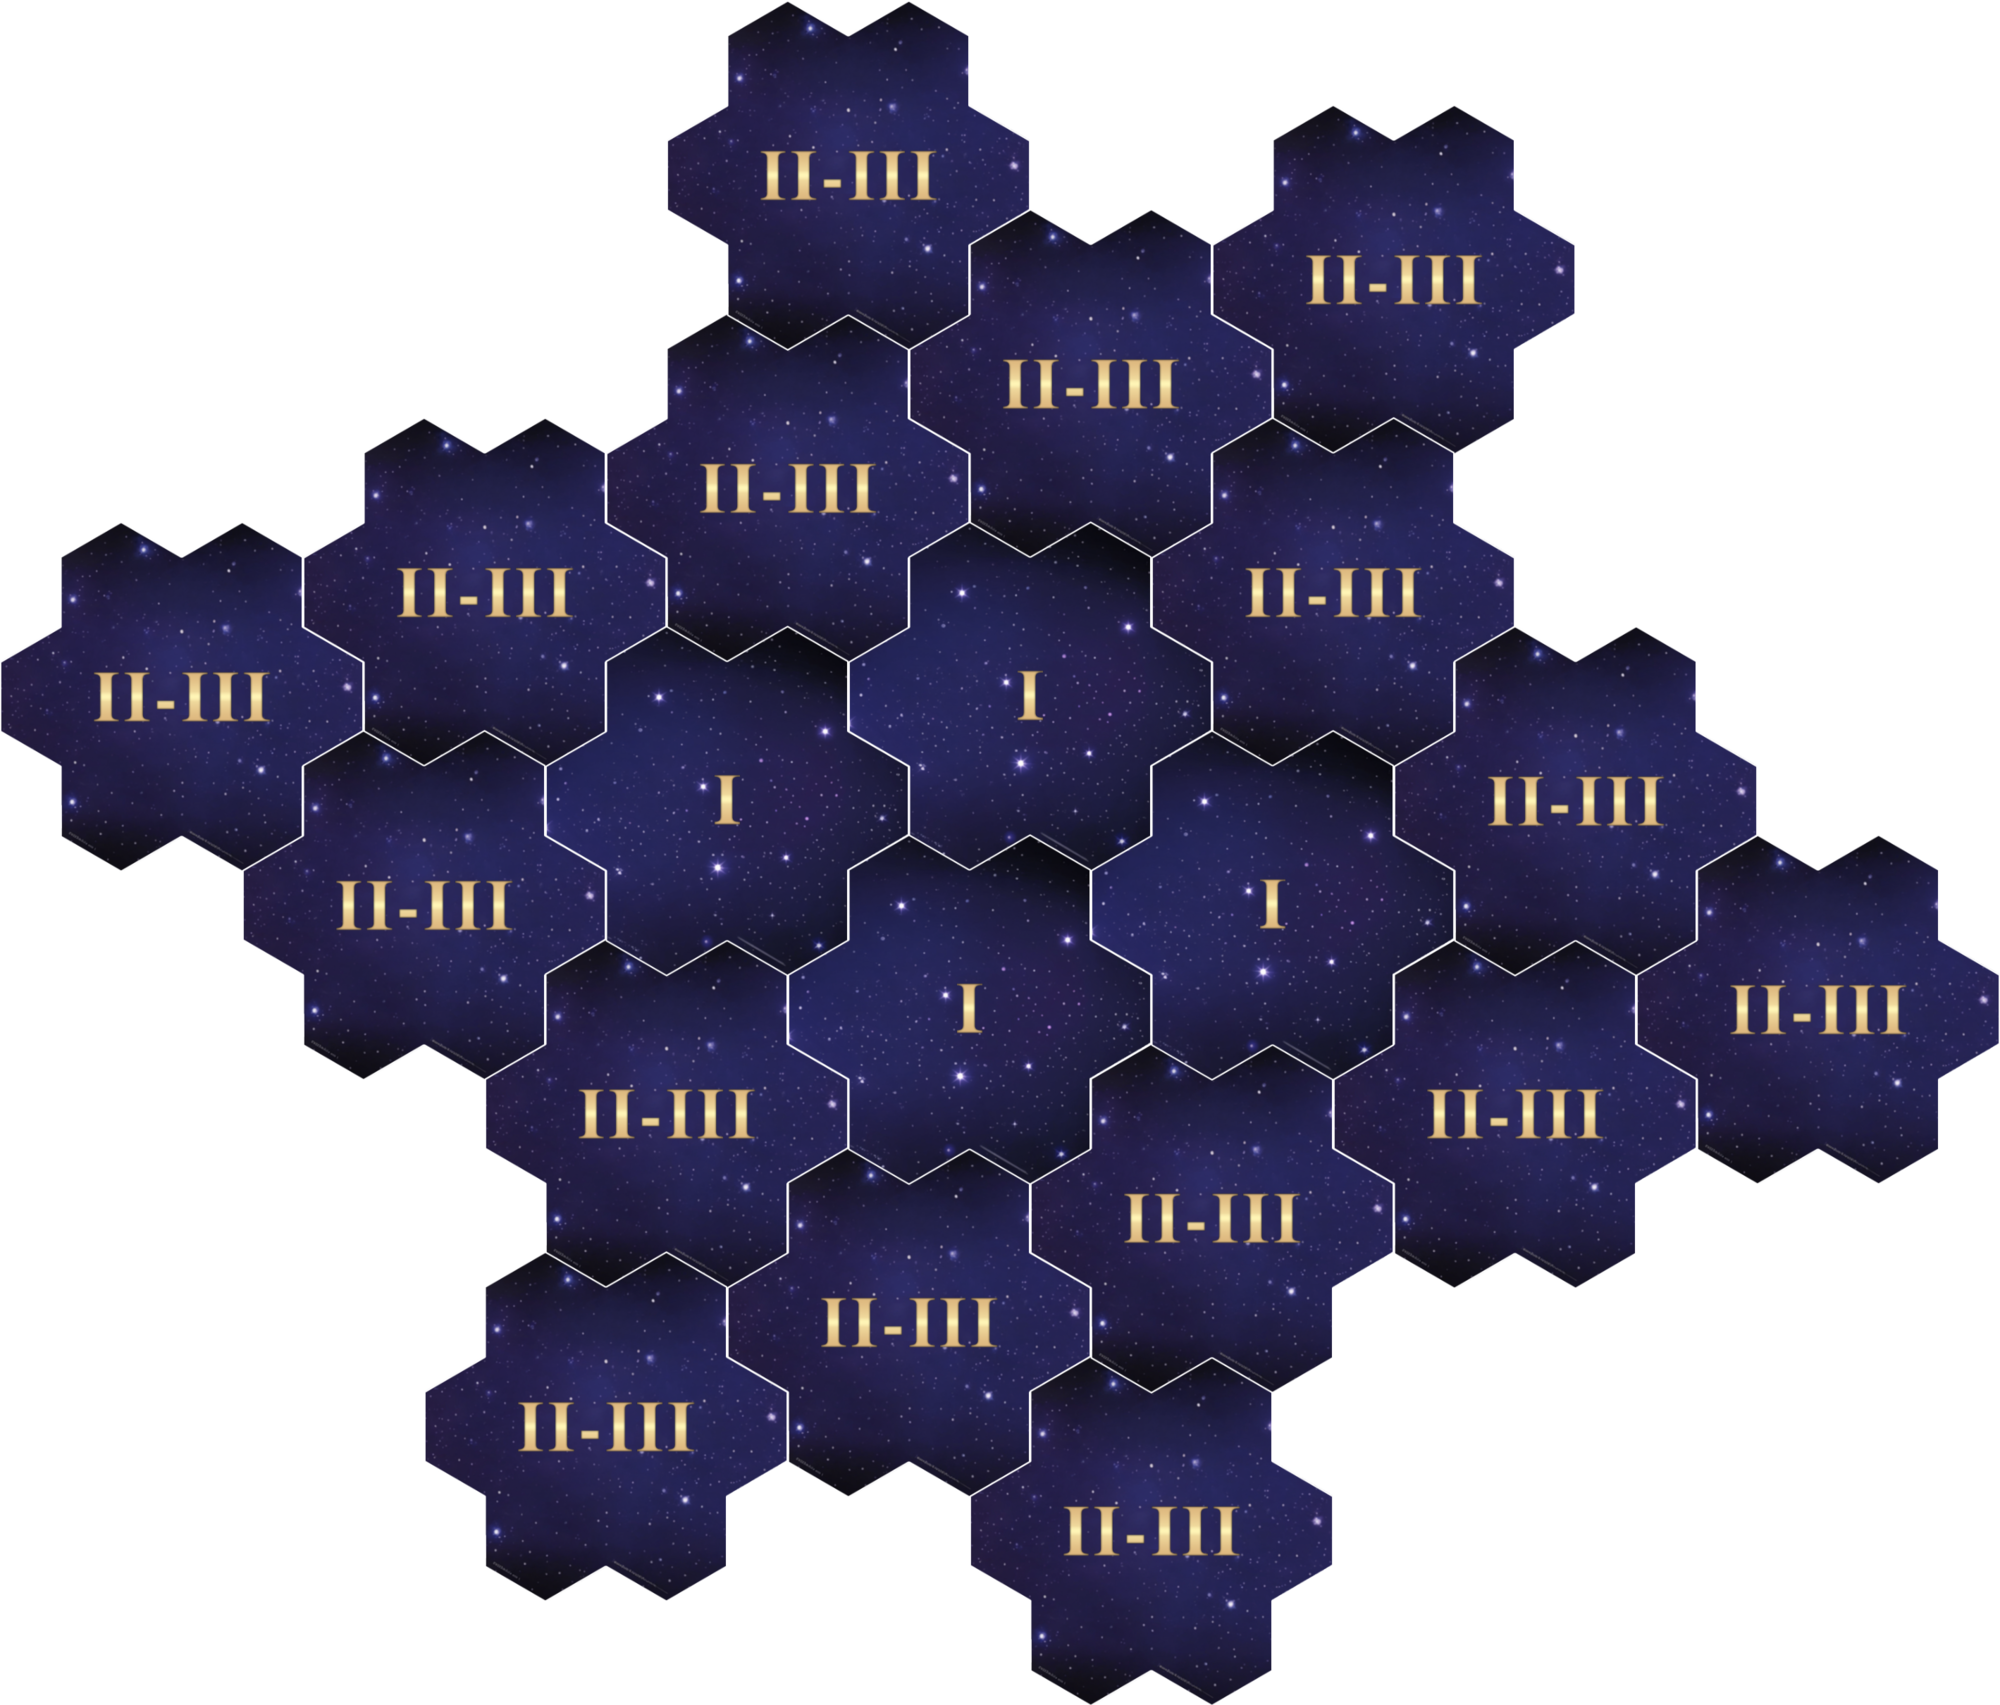
\includegraphics[width=0.3\paperwidth]{\_assets/maps/emerald-4.png}
  \captionof{figure}{4-PLAYER SCENARIO}
\end{center}

\end{multicols*}
